\documentclass[journal]{IEEEtran}

\usepackage{amsmath,amsfonts,amssymb,bm}
\usepackage{algorithmic}
\usepackage{algorithm}
\usepackage{array}
\usepackage{booktabs}
\usepackage[caption=false,font=normalsize,labelfont=sf,textfont=sf]{subfig}
\usepackage{textcomp}
\usepackage{url}
\usepackage{verbatim}
\usepackage{graphicx}
\usepackage{multirow}
\usepackage{cite}
\hyphenation{op-tical net-works semi-conduc-tor}
\graphicspath{{../figures/}{../figures/scenes/}{../figures/paper/}}

\newcommand{\method}{\textsc{GFA}}

\begin{document}

\title{Grounded Factor Abstraction for Decision-Sufficient Driving World Models}

\author{First~Author,
        Second~Author,
        and~Corresponding~Author%
\thanks{Manuscript draft prepared on April 23, 2026. Replace this note with the final submission metadata before submission.}%
\thanks{First Author, Second Author, and Corresponding Author are with the authors' institution and research lab. Replace affiliations, city, and postal code before submission.}%
\thanks{Corresponding author: corresponding.author@example.com}}

\maketitle

\begin{abstract}
Relation-aware world models are appealing for autonomous driving, but most current formulations treat objects and relations as exchangeable scene tokens under a shared latent bottleneck. We argue that this formulation is conceptually fragile: dynamic objects are state-bearing variables whose future must be rolled out, whereas interactions are grounded factors whose meaning depends on the retained entities they connect. When interaction cues are represented as free-floating tokens, a limited-capacity world model may select interaction evidence while missing its endpoint entities, producing ungrounded interaction factors and degrading decision-relevant prediction. We present \method, a grounded factor abstraction that first retains dynamic state variables and then attaches decision-relevant interaction factors to the retained entities. In our implementation, this grounding principle is instantiated as a fixed-slot abstraction with separate entity and factor capacities; the specific top-$K$ operator is an implementation of the capacity constraint, not the scientific problem itself. Under a fair 16-slot budget on nuScenes, \method\ reduces rare-agent displacement error by 55.2\% and improves interaction recall at 1\,m by 8.3 points over an object-only baseline, while a free-floating object-relation token baseline collapses. On planning-oriented nuPlan, the same grounded abstraction yields the strongest 20k and 50k latent-policy results. At 50k, it achieves $14.51 \pm 2.93$ return and $0.259 \pm 0.045$ collision rate, versus $1.72 \pm 17.89$ and $0.610 \pm 0.146$ for object-only; an offline planner-like probe also shows lower teacher-action error ($6.63 \pm 0.11$ versus $8.86 \pm 0.37$). Mechanistic diagnostics, interaction-semantic ablations, and interaction-conditioned subsets support the same conclusion: decision-sufficient driving representations should ground interaction factors on retained state-bearing entities rather than treating relations as independent tokens.
\end{abstract}

\begin{IEEEkeywords}
Autonomous driving, world models, grounded interaction factors, decision-sufficient representation, policy learning.
\end{IEEEkeywords}

\section{Introduction}
\IEEEPARstart{W}{orld} models offer an appealing route to autonomous driving policy learning because they replace expensive environment interaction with imagined trajectories \cite{ha2018worldmodels,hafner2023dreamerv3}. For driving, this promise is especially attractive: direct policy optimization is expensive, safety-critical, and often bottlenecked by sparse feedback. At the same time, a driving policy must reason about a small number of highly consequential entities and their interactions rather than an undifferentiated global state.

This tension raises a representation question that is still under-specified in the current literature: \emph{what should be a latent variable in a fixed-capacity driving world model, and what should be a factor conditioned on those variables?} A common implementation answer is to append relation tokens to the same selection bottleneck used for dynamic agents. However, that design implicitly treats objects and interactions as exchangeable units of capacity. In autonomous driving, this assumption is brittle. A lane-conflict or time-to-collision cue is meaningful only when the dynamic agent involved in that interaction is still represented in the latent state.

We study this problem through the lens of grounded factorization. Our central claim is that relation-aware driving world models fail or succeed not only because of what interaction information they encode, but also because of \emph{whether that information is grounded on retained state-bearing entities}. This motivates \method, a grounded factor abstraction for limited-capacity driving world models. The design first retains dynamic entities as latent state variables and then attaches interaction factors to those retained entities. In the current implementation, the capacity constraint is realized with separate entity and factor slots; conceptually, however, the key point is the grounding constraint rather than the particular top-$K$ operator.

The second question is whether representation gains translate to policy learning. Better forecasting metrics do not automatically imply a better control landscape for latent-space policy optimization. We therefore organize the paper in two stages. Stage 0 studies representation sufficiency under a fair 16-slot latent bottleneck on nuScenes. Stage 1 studies imagination-based policy learning across two downstream regimes: nuScenes short-horizon latent imagination and a planning-oriented nuPlan preprocessed benchmark. This split allows us to ask not only whether grounded factor abstraction is useful, but also when it becomes actionable for policy optimization.

The resulting picture is more nuanced and, we believe, more valuable than a simple ``method always wins'' story. On nuScenes, Stage 0 strongly favors the grounded factor representation, but Stage 1 still prefers the object-only policy baseline. On nuPlan 20k and its 50k scale-up, however, the ranking flips: the no-visibility grounded-factor variant becomes the most reliable policy-learning condition, and an additional offline planner-like sanity probe supports the same choice. Cross-dataset transfer rollouts and horizon-sensitivity diagnostics point to the same conclusion. This shows that interaction factors are not a universal free lunch. Their benefit depends on whether the downstream planning regime and tokenization characteristics make the grounded interaction structure actionable for policy learning.

Under this scope, the paper is not a full end-to-end perception-to-control system and not yet a full external closed-loop benchmark paper. It is a method-and-analysis paper about decision-sufficient semantic abstraction for imagination-based driving policy learning. That narrower framing is deliberate: it lets us isolate the representation-policy interface before introducing additional confounders such as perception noise or simulator-specific artifacts.

Figure~\ref{fig:teaser} summarizes this overall story: a fixed-capacity failure mode caused by free-floating interactions, a structural fix through grounded entity-factor abstraction, and a downstream ranking reversal that only appears once the planning regime makes interaction factors actionable.

The contributions of this paper are as follows.
\begin{enumerate}
\item We identify \emph{ungrounded interaction factors} as a failure mode of relation-aware latent driving models: free-floating relation evidence can occupy limited capacity while the state-bearing endpoint entity is absent.
\item We propose \method, a decision-sufficient factorized abstraction that retains dynamic entities as latent variables and grounds interaction factors on those retained entities while keeping the total world-model context fixed.
\item We introduce mechanism diagnostics for critical entity retention and ungrounded factor rate, linking representation failures to rare-agent prediction and interaction recall.
\item We show that grounded factor abstraction improves representation sufficiency on nuScenes, but its downstream policy-learning benefit is dataset-dependent: object-only remains the most stable baseline on nuScenes Stage 1, whereas the no-visibility grounded-factor variant becomes the robust winner on nuPlan 20k/50k, in downstream offline planner-like probes, and in follow-up transfer diagnostics.
\end{enumerate}

\begin{figure*}[!t]
\centering

\includegraphics[width=0.98\textwidth]{paper/fig1.png}
\caption{Teaser figure summarizing the paper's core story. Under a fixed 16-slot latent bottleneck, free-floating interaction tokens can displace decision-critical dynamic agents and become ungrounded; grounded factor abstraction restores state-bearing context before injecting interaction evidence; and the resulting policy-learning benefit appears only in downstream regimes where interaction structure becomes actionable.}
\label{fig:teaser}
\end{figure*}

\section{Related Work}
\subsection{World Models for Driving Policy Learning}
World models have become a central approach to imagination-based policy learning \cite{ha2018worldmodels,hafner2023dreamerv3}. In driving, they promise to replace expensive simulator interaction with learned latent rollouts. Yet most formulations focus on latent prediction efficiency rather than on the semantic status of the variables being rolled out. Our work addresses that missing question directly: dynamic agents should be treated as state-bearing variables, while interaction cues should be treated as factors grounded on those variables.

\subsection{Object-Centric and Relational Representations}
Object-centric learning \cite{locatello2020slotattention} has shown that scenes composed of interacting entities benefit from structured representations. Autonomous driving inherits this need: policies must reason about nearby vehicles, vulnerable road users, and interaction cues such as right-of-way, lane conflict, and time-to-collision. Prior work has established that object, map, and relational structure help prediction and planning. We extend that line by separating two roles that are often conflated: objects are latent state variables to be predicted forward, whereas relations are interaction factors whose meaning depends on the entities they connect.

\subsection{Driving Benchmarks and Cross-Dataset Evaluation}
nuScenes \cite{caesar2020nuscenes} and nuPlan \cite{caesar2021nuplan} provide two complementary views of driving data: the former is widely used for perception and trajectory modeling, whereas the latter is more directly aligned with planning evaluation. Additional platforms such as CARLA \cite{dosovitskiy2017carla}, World on Rails \cite{chen2021worldonrails}, Waymax \cite{mao2023waymax}, and NAVSIM \cite{dauner2024navsim} further emphasize that downstream task setting matters. Our experiments leverage this contrast directly: the same representation can look very different once it is used for imagination-based policy learning under different planning regimes.

\section{Problem Formulation}
We consider a driving agent acting in a partially observable traffic environment. At time step $t$, the agent receives a structured scene representation
\begin{equation}
\mathbf{x}_t = \{\mathbf{e}_t, \mathcal{O}_t, \mathcal{M}_t, \Phi_t\},
\label{eq:state}
\end{equation}
where $\mathbf{e}_t$ denotes the ego state, $\mathcal{O}_t=\{o_{t,i}\}$ denotes dynamic state-bearing entities, $\mathcal{M}_t$ denotes map context, and $\Phi_t=\{\phi_{t,ij}\}$ denotes interaction factors such as TTC, risk, lane conflict, and priority. The policy $\pi(\mathbf{a}_t \mid \mathbf{x}_t)$ outputs a driving action $\mathbf{a}_t$, which may correspond to low-level control or a compact motion command.

The world model cannot consume the full scene indefinitely. It must compress $\mathbf{x}_t$ into a latent context of fixed capacity $K$. The central problem studied in this paper is therefore not only \emph{what} information to encode, but also \emph{what is allowed to exist independently in the latent state}. Dynamic entities carry physical state and must be rolled forward. Interaction factors are conditional evidence: a factor $\phi_{t,ij}$ is meaningful only when the relevant endpoint entity remains available to ground it. Our objective is to learn an abstraction $A_\theta$ and world model $f_\theta$ such that the resulting latent state remains decision-sufficient for two downstream tasks:
\begin{enumerate}
\item \textbf{Representation sufficiency:} preserve dynamic prediction, rare-agent tracking, and interaction-critical structure under a fair fixed latent budget.
\item \textbf{Policy learning:} support stable imagination-based policy optimization.
\end{enumerate}

This formulation deliberately separates the conceptual problem from one particular selector. A top-$K$ bottleneck is one way to instantiate fixed capacity, but the more general failure is an \emph{ungrounded factor}: interaction evidence is retained while the state-bearing entity needed to interpret it is absent. Conversely, a decision-sufficient abstraction should first retain the critical entity state and then attach interaction factors to the retained state.

\subsection{Scope and Evaluation Assumptions}
This work studies decision learning under structured scene tokens rather than full end-to-end perception. We assume \emph{oracle-token evaluation}: scene tokens are derived from annotations, simulator state, or an equivalent trusted front-end. This assumption is intentional. It isolates the abstraction-and-policy question from perception noise and allows us to compare downstream planning regimes directly. The resulting paper should therefore be read as a study of latent representation and imagination-based policy learning, not as a claim about complete perception-to-control autonomy.

\section{Method}
\subsection{Scene Factorization}
Each scene is represented in an ego-centric local frame to encourage cross-benchmark consistency. The raw feature layout used by the current implementation contains a fixed-length vector of dimension $D_{\mathrm{raw}}=40$, with the first coordinates reserved for relative position, velocity, object extent, risk proxies, visibility, time-to-collision, lane conflict, interaction priority, distance, heading, and serialized type. The maximum serialized context is $S=97$, corresponding to one ego entry, a bounded set of dynamic-object entries, map entries, relation-feature entries, and padding.

This implementation still serializes the scene as tokens for compatibility with existing world-model code, but the semantics are factorized. Dynamic-object entries represent state-bearing entities with physical next states. Relation-feature entries represent interaction factors: pairwise or ego-agent cues such as relative position, relative velocity, distance, time-to-collision proxy, lane conflict indicator, visibility or occlusion score, and interaction priority. These factors should not be interpreted as standalone objects with independent physical rollouts; they are evidence attached to retained entities.

The serialized schema is shared across the two main Stage-1 regimes, but the factor statistics are not. nuScenes factors are generated from annotated driving scenes with visibility variation, whereas the nuPlan preprocessed pipeline materializes one NPZ anchor frame per sample and the official nuPlan closed-loop adapter recomputes interaction factors online from current ego and tracked-object geometry. In that adapter, interaction factors are constructed from relative geometry, relative velocity, TTC, lane conflict, risk, and priority heuristics, while visibility is effectively constant. This difference is useful later when interpreting why visibility weighting behaves differently on nuScenes and nuPlan.

\subsection{Grounded Factor Abstraction}
Given token features $\mathbf{x}_{t,i}$ and token types $c_{t,i}$, an encoder produces latent token embeddings
\begin{equation}
\mathbf{h}_{t,i} = g_{\mathrm{enc}}(\mathbf{x}_{t,i}, c_{t,i}),
\label{eq:encoder}
\end{equation}
where $g_{\mathrm{enc}}$ is implemented as a token encoder with learned type embeddings. A capacity-limited abstraction module scores candidates using ego-conditioned attention:
\begin{equation}
\alpha_{t,i} = \mathrm{softmax}_i\left(\frac{(\mathbf{W}_q \mathbf{h}_{t,\mathrm{ego}})^\top(\mathbf{W}_k \mathbf{h}_{t,i})}{\sqrt{d}}\right),
\label{eq:attention}
\end{equation}
followed by a learned importance head
\begin{equation}
s_{t,i} = g_{\mathrm{score}}([\mathbf{h}_{t,i}; \alpha_{t,i}]).
\label{eq:score}
\end{equation}
The implementation uses top-$K$ selection to instantiate a fixed 16-slot capacity. This operator is not the core contribution; it is the experimental bottleneck that lets us test whether interaction information is grounded correctly. A pooled global latent $\mathbf{z}^{\mathrm{glob}}_t$ is computed in parallel for policy evaluation and value prediction.

This abstraction is not merely a compression stage. It acts as a decision bottleneck: if the representation fails to retain safety-critical interactive structure, the downstream policy should degrade in precisely the scenarios that matter to driving. Our experimental design therefore treats representation sufficiency as a central scientific question rather than a minor implementation detail.

In the final \method\ instantiation used in our Stage-0 representation study, we enforce grounding through a two-part abstraction. First, a state path selects dynamic entities
\begin{equation}
S_{\mathrm{ent}} = A_{\mathrm{ent}}(\mathcal{O}_t), \quad |S_{\mathrm{ent}}| \le K_{\mathrm{ent}}.
\label{eq:entity}
\end{equation}
Second, a factor path selects interaction evidence only as factor information associated with retained or retainable entities,
\begin{equation}
S_{\mathrm{fac}} = A_{\mathrm{fac}}(\Phi_t \mid S_{\mathrm{ent}}), \quad |S_{\mathrm{fac}}| \le K_{\mathrm{fac}}.
\label{eq:factor}
\end{equation}
The total capacity is unchanged:
\begin{equation}
K_{\mathrm{ent}} + K_{\mathrm{fac}} = K.
\label{eq:capacitysplit}
\end{equation}
The world model then receives selected entity slots together with grounded factor slots. Under the fair 16-slot budget used in our experiments, we instantiate this as $(K_{\mathrm{ent}}, K_{\mathrm{fac}}) = (12,4)$. This design is motivated by a simple failure mode: when interaction factors are represented as independent tokens inside a shared bottleneck, they may displace the dynamic-agent states required to interpret them. The grounded formulation preserves the total context size while preventing free-floating factors from replacing state-bearing entities.

Figure~\ref{fig:method_overview} is intended to make this distinction visually explicit by contrasting free-floating object-relation selection with grounded entity-factor abstraction inside the same overall world-model pipeline.

\begin{figure*}[!t]
\centering

\includegraphics[width=0.98\textwidth]{paper/fig2.png}
\caption{Method overview of \method. The figure contrasts naive free-floating object-relation selection with the proposed grounded entity-factor path, annotates the fair $(12,4)$ entity/factor capacity split inside the shared 16-slot bottleneck, and shows how the selected slots feed the action-conditioned latent dynamics model and imagination-based policy/value optimization loop.}
\label{fig:method_overview}
\end{figure*}

\subsection{Reactive Object-Relational World Model}
The world model receives the selected token set $\mathbf{z}^{\mathrm{sel}}_t$ and action $\mathbf{a}_t$, then predicts next-step latent entities, reward, continuation probability, and collision risk:
\begin{equation}
\hat{\mathbf{z}}^{\mathrm{sel}}_{t+1}, \hat{r}_t, \hat{c}_t, \hat{\rho}_t =
f_\theta(\mathbf{z}^{\mathrm{sel}}_t, \mathbf{a}_t).
\label{eq:worldmodel}
\end{equation}
The action is injected into token dynamics so that predicted transitions can depend on ego intervention. This is essential: without action-conditioned multi-agent prediction, the latent model would regress toward a sophisticated replay predictor rather than a reactive closed-loop model.

The training loss combines next-token prediction, reward prediction, continuation prediction, and auxiliary collision-risk prediction:
\begin{equation}
\mathcal{L}_{\mathrm{wm}} =
\lambda_{\mathrm{obs}}\mathcal{L}_{\mathrm{obs}} +
\lambda_{r}\mathcal{L}_{r} +
\lambda_{c}\mathcal{L}_{c} +
\lambda_{\mathrm{col}}\mathcal{L}_{\mathrm{col}}.
\label{eq:wmloss}
\end{equation}
The current scaffold also allows an optional behavior-cloning regularizer during warm start,
\begin{equation}
\mathcal{L} = \mathcal{L}_{\mathrm{wm}} + \lambda_{\mathrm{bc}}\mathcal{L}_{\mathrm{bc}} + \mathcal{L}_{\mathrm{pol}},
\label{eq:totalloss}
\end{equation}
which stabilizes early training when the world model and value function are still inaccurate.

\subsection{Latent Imagination Policy Learning}
We optimize a policy-and-value stack on imagined trajectories produced by the world model. At each rollout step, the policy head reads $\mathbf{z}^{\mathrm{glob}}_t$ and outputs the parameters of a continuous diagonal-Gaussian action distribution. To prevent imagination training from exploding numerically, the action mean is bounded with a scaled hyperbolic tangent and the log standard deviation is clamped to a finite interval before sampling. A value head estimates state value from the same global latent. In Stage 1, we use a 5-step latent rollout, GAE-$\lambda$ targets, reward clipping, detached world-model updates during policy optimization, and a real-batch sanity loss that keeps the representation grounded. The purpose of this stage is not to claim a new optimization algorithm, but to test whether a representation that looks stronger in Stage 0 also produces a more favorable optimization landscape for imagination-based policy learning.

The resulting training procedure is summarized in Algorithm~\ref{alg:gfa}. Compared with render-in-the-loop optimization, this design keeps policy improvement in latent space and lets us study directly whether semantic abstraction quality changes the stability of downstream policy optimization.

\begin{algorithm}[!t]
\caption{\method\ Policy-Learning Procedure}
\label{alg:gfa}
\begin{algorithmic}[1]
\STATE Collect or load structured scene transitions from offline data and reactive rollouts.
\STATE Encode state-bearing entities and grounded interaction factors.
\STATE Update the world model using $\mathcal{L}_{\mathrm{wm}}$ in (\ref{eq:wmloss}).
\STATE Warm start the policy with behavior cloning if expert actions are available.
\STATE Roll out imagined latent trajectories with the current policy and world model.
\STATE Update the policy and value heads using imagined rewards, continuation, and value targets.
\STATE Periodically evaluate the policy in external closed-loop benchmarks.
\STATE Keep the final model based on external evaluation rather than latent-only validation.
\end{algorithmic}
\end{algorithm}

\section{Experimental Design}
\subsection{Research Questions}
The experiments are organized around four questions that mirror the paper's definition of decision-sufficient grounded abstraction:
\begin{enumerate}
\item \textbf{RQ1: Representation sufficiency.} Does grounded entity-factor abstraction preserve dynamic agents and interaction-critical structure under the same latent capacity?
\item \textbf{RQ2: Mechanism.} Does the free-floating relation baseline fail by retaining ungrounded interaction evidence while missing critical state-bearing entities?
\item \textbf{RQ3: Planning transfer.} When a representation is stronger, does it produce a better latent policy across nuScenes and nuPlan planning regimes?
\item \textbf{RQ4: Interaction specificity.} Are the gains concentrated in scenes and factor dimensions where interaction reasoning should matter?
\end{enumerate}

\subsection{Datasets, Variants, and Metrics}
Table~\ref{tab:protocols} summarizes the protocols. Stage 0 isolates representation quality under a fair 16-slot bottleneck. Stage 1 evaluates whether the learned abstraction changes the optimization landscape of imagination-based policy learning. nuScenes is used as a compact, visibility-rich scene benchmark; nuPlan is used as the planning-oriented scale-up where interaction factors are more directly tied to teacher actions.

\begin{table}[!t]
\caption{Experimental protocols. The main paper uses latent and offline planner-like probes to isolate representation and policy-learning behavior before claiming full closed-loop benchmark performance.}
\label{tab:protocols}
\centering
\resizebox{\columnwidth}{!}{%
\begin{tabular}{lll}
\toprule
Protocol & Dataset and Split & Role \\
\midrule
Stage 0 & nuScenes, 700 scenes & Representation sufficiency \\
Stage 1A & nuScenes, 700 scenes & Short-horizon latent policy \\
Stage 1B & nuPlan 20k, 16k/4k & Planning-oriented policy \\
Stage 1C & nuPlan 50k, 40k/10k & Scale-up and downstream probes \\
\bottomrule
\end{tabular}}
\end{table}

The variants are chosen to separate capacity, relation serialization, and grounding. \textbf{Object-Only} keeps only state-bearing dynamic entities. \textbf{Object+Relation} is the free-floating baseline that serializes relation features as ordinary selectable entries. \textbf{\method} retains entity state and factor evidence through separate entity/factor capacities, implemented as a 12/4 split under the same total 16 slots. \textbf{\method+Visibility} adds visibility weighting on the entity path. Stage 1 reports \texttt{wm\_object}, \texttt{wm\_decoupled}, and \texttt{wm\_decoupled\_no\_vis}, plus a free-floating \texttt{wm\_naive} row on nuPlan 20k and a low-cost BC/planner-imitation anchor on nuPlan 50k.

Stage 0 reports dynamic rollout MSE, collision F1, rare-agent ADE, and Interaction Recall@1m. Mechanism diagnostics report Critical Dynamic Retention (CDR), MissRate, WastedRel, and relation over-allocation index (ROI). Stage 1 reports latent return, imagined collision rate, collision mean, and ego-latent stability. Downstream nuPlan probes additionally report teacher-action MSE and action $\Delta L_2$.

\subsection{Implementation Details}
The shared model configuration uses raw dimension $40$, model dimension $128$, hidden dimension $256$, four attention heads, two transformer world-model layers, and a serialized scene budget of $97$. The fair compact setting uses $K=16$ latent slots. Stage 0 uses Adam with learning rate $10^{-3}$, batch size $32$, $15$ epochs, and three seeds $\{7,42,2026\}$. Stage 1 uses a 5-step imagination horizon, batch size $128$, learning rate $4\times 10^{-3}$, $10$ epochs, three seeds $\{7,42,123\}$, GAE-$\lambda$ targets with $(\gamma,\lambda)=(0.97,0.95)$, reward clipping to $[-5,5]$, a Huber critic, detached world-model updates, and bounded action statistics.

\section{Results}
\subsection{RQ1: Grounded Factors Improve Fixed-Capacity Representation}
Table~\ref{tab:repr_ablation} is the main representation result. The fair comparison keeps the world-model context fixed at 16 slots. The 97-token holistic model is treated as a non-fair upper bound and discussed only as headroom.

\begin{table*}[!t]
\caption{Stage-0 representation sufficiency on nuScenes under a fair 16-slot world-model context. All results are averaged over three seeds; $\pm$ denotes seed standard deviation.}
\label{tab:repr_ablation}
\centering
\resizebox{\textwidth}{!}{%
\begin{tabular}{lccccc}
\toprule
Representation & Ctx & Dyn Rollout $\downarrow$ & Collision F1 $\uparrow$ & Rare ADE $\downarrow$ & IntRec@1m $\uparrow$ \\
\midrule
Holistic-16Slot & 16 & $2.11 \pm 0.16$ & $0.978 \pm 0.011$ & $1.42 \pm 0.01$ & $0.643 \pm 0.015$ \\
Object-Only-16 & 16 & $3.74 \pm 1.01$ & $0.946 \pm 0.004$ & $1.10 \pm 0.12$ & $0.901 \pm 0.034$ \\
Object+Relation-16 (free-floating) & 16 & $40.28 \pm 29.54$ & $0.980 \pm 0.013$ & $7.51 \pm 5.48$ & $0.430 \pm 0.407$ \\
Object+Relation+Visibility-16 & 16 & $15.80 \pm 9.93$ & $0.933 \pm 0.064$ & $2.96 \pm 1.64$ & $0.728 \pm 0.155$ \\
\midrule
\textbf{\method\ Entity+Factor} & 16 & $2.11 \pm 0.19$ & $0.929 \pm 0.039$ & $\mathbf{0.49 \pm 0.18}$ & $\mathbf{0.984 \pm 0.014}$ \\
\textbf{\method+Visibility} & 16 & $\mathbf{1.88 \pm 0.23}$ & $0.926 \pm 0.029$ & $0.52 \pm 0.05$ & $0.979 \pm 0.008$ \\
\midrule
$\Delta$ \method\ vs Object-Only & -- & $-43.5\%$ & $-1.8$ pts & $-55.2\%$ & $+8.3$ pts \\
$\Delta$ \method+Vis vs Object-Only & -- & $-49.9\%$ & $-2.1$ pts & $-52.6\%$ & $+7.8$ pts \\
\bottomrule
\end{tabular}}
\end{table*}

The central result is not that adding serialized relations is always helpful. The opposite is true: the free-floating Object+Relation baseline collapses, increasing rare-agent ADE from $1.10$ to $7.51$ and reducing Interaction Recall@1m from $0.901$ to $0.430$. The same interaction evidence becomes useful only when it is grounded on retained state-bearing entities. \method\ reduces rare-agent ADE by $55.2\%$ relative to Object-Only and improves Interaction Recall@1m by $8.3$ points. \method+Visibility gives the best dynamic rollout MSE, but the later planning results show that visibility is dataset-conditional rather than a universal improvement.

\subsection{RQ2: Free-Floating Relations Fail Through Ungrounded Factors}
The mechanism claim is that the naive relation formulation spends limited capacity on interaction evidence without preserving the entity state needed to interpret it. Table~\ref{tab:grounding_diagnostics} reports this directly. CDR measures how often critical dynamic entities are retained; WastedRel measures selected interaction factors whose non-ego endpoint is absent from the retained state.

\begin{table}[!t]
\caption{Mechanism diagnostics for grounded factorization.}
\label{tab:grounding_diagnostics}
\centering
\resizebox{\columnwidth}{!}{%
\begin{tabular}{lcccc}
\toprule
Condition & CDR $\uparrow$ & MissRate $\downarrow$ & WastedRel $\downarrow$ & ROI \\
\midrule
WM-Naive-Shared & $0.547$ & $0.453$ & $0.216$ & $0.054$ \\
WM-Object & $0.785$ & $0.215$ & -- & $0.000$ \\
\textbf{WM-Decoupled-NoVis} & $\mathbf{0.939}$ & $\mathbf{0.061}$ & $\mathbf{0.044}$ & $0.260$ \\
\bottomrule
\end{tabular}}
\end{table}

\begin{figure*}[!t]
\centering

\includegraphics[width=\textwidth]{paper_stage0_slot_budget.pdf}
\caption{Stage-0 slot-type composition. The free-floating relation baseline spends compact context on relation-feature entries and starves nearby dynamic agents. Grounded factor variants preserve entity coverage while reserving factor capacity.}
\label{fig:slot_distribution}
\end{figure*}

\begin{figure*}[!t]
\centering
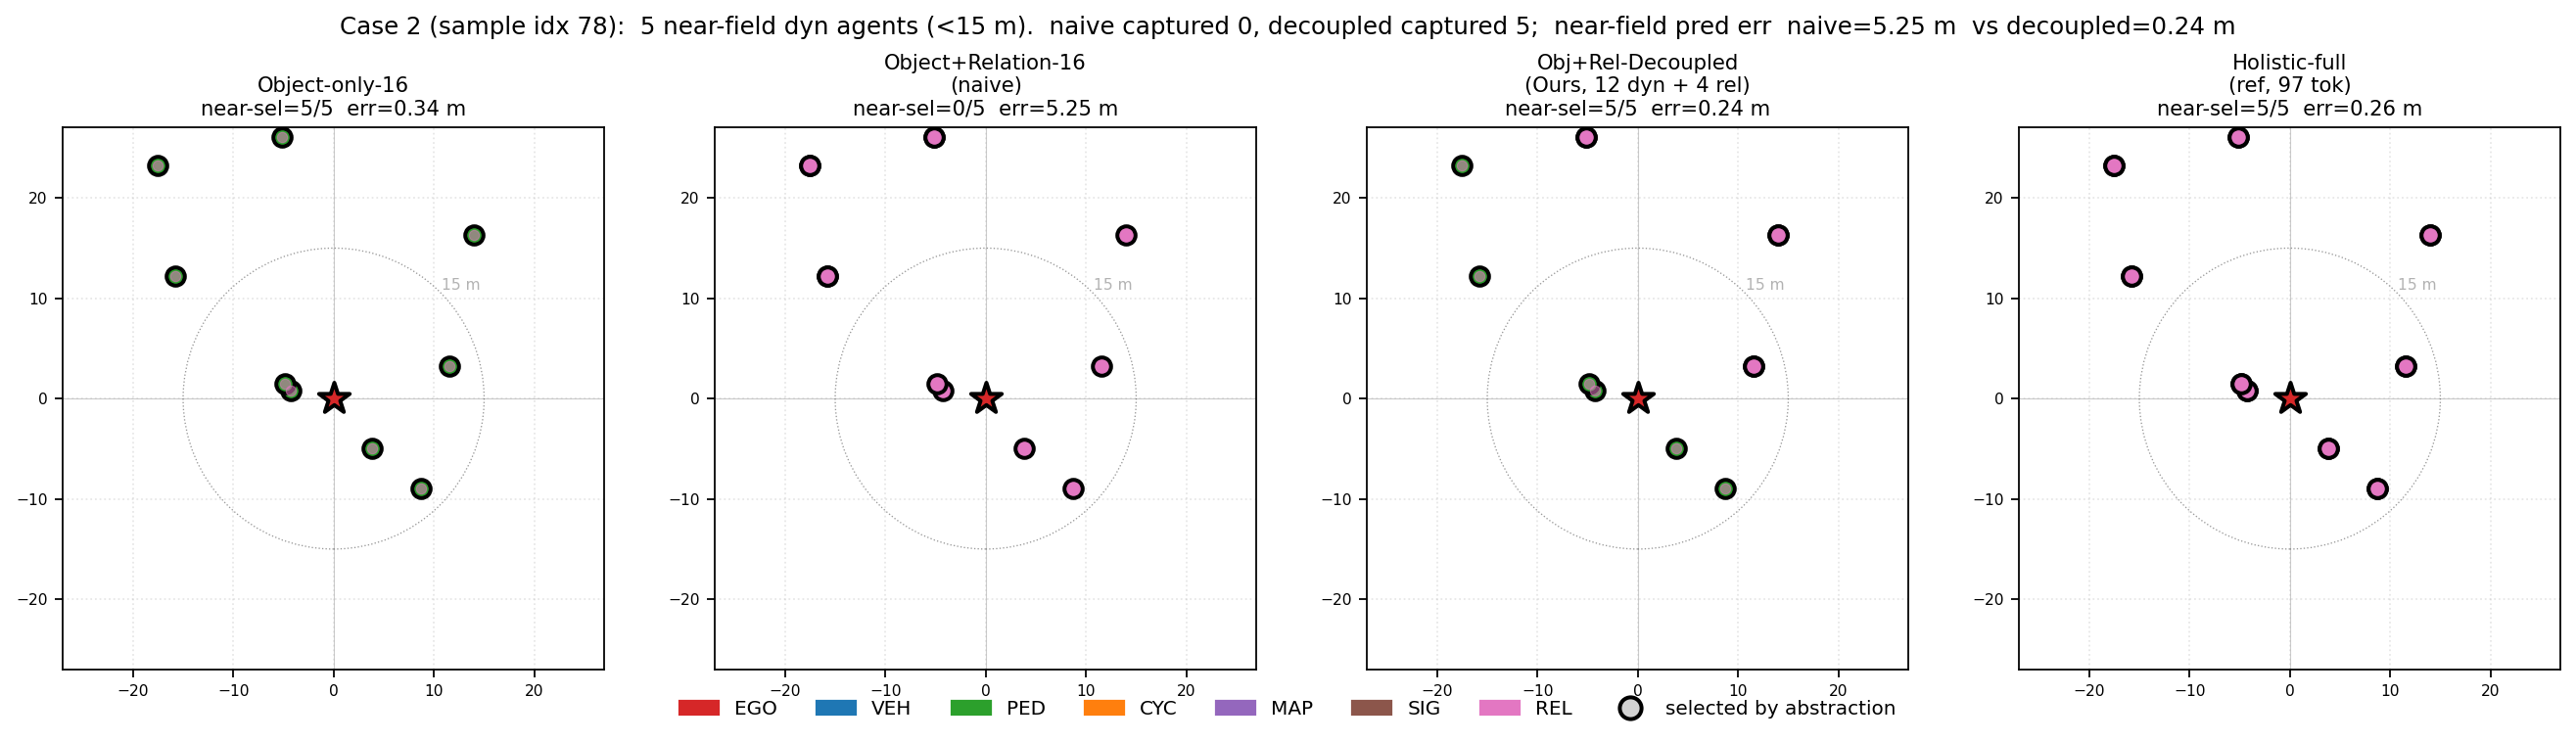
\includegraphics[width=\textwidth]{case_02_idx78.png}
\caption{Qualitative fixed-capacity abstraction case. The naive Object+Relation-16 variant captures none of five near-field dynamic agents within 15\,m and incurs 5.25\,m near-field prediction error. The grounded entity-factor variant captures all five and reduces the error to 0.24\,m under the same compact budget.}
\label{fig:qualitative}
\end{figure*}

The diagnostics match the failure definition. WM-Naive-Shared retains only $54.7\%$ of critical dynamic entities and wastes $21.6\%$ of selected relation factors. WM-Decoupled-NoVis raises CDR to $93.9\%$ and reduces WastedRel to $4.4\%$. Fig.~\ref{fig:slot_distribution} and Fig.~\ref{fig:qualitative} provide visual evidence for the same mechanism: the model does not fail because interaction cues are meaningless, but because they become ungrounded when endpoint state is missing.

\subsection{RQ3: Representation Gains Transfer Conditionally to Planning}
Table~\ref{tab:stage1_cross_dataset} evaluates imagination-based policy learning. This is the main downstream table, and it deliberately reports both positive and negative results.

\begin{table*}[!t]
\caption{Stage-1 imagination-based policy learning across datasets and nuPlan scales. Results are averaged over three seeds. Ego stability is a divergence sentinel rather than the row-ranking criterion.}
\label{tab:stage1_cross_dataset}
\centering
\resizebox{\textwidth}{!}{%
\begin{tabular}{llcccc}
\toprule
Dataset & Condition & Return $\uparrow$ & Coll. Rate $\downarrow$ & Coll. Mean $\downarrow$ & Ego Stability \\
\midrule
nuScenes & \textbf{WM-Object} & $\mathbf{31.79 \pm 19.70}$ & $\mathbf{0.597 \pm 0.048}$ & $\mathbf{0.610 \pm 0.048}$ & $0.258 \pm 0.058$ \\
nuScenes & WM-Decoupled & $4.34 \pm 13.66$ & $0.695 \pm 0.283$ & $0.676 \pm 0.243$ & $0.636 \pm 0.108$ \\
nuScenes & WM-Decoupled-NoVis & $0.34 \pm 15.97$ & $0.820 \pm 0.260$ & $0.814 \pm 0.167$ & $0.223 \pm 0.033$ \\
\midrule
nuPlan 20k & WM-Object & $4.74 \pm 13.95$ & $0.373 \pm 0.083$ & $0.395 \pm 0.057$ & $0.426 \pm 0.099$ \\
nuPlan 20k & WM-Naive-Shared & $-2.66 \pm 14.63$ & $0.252 \pm 0.050$ & $0.297 \pm 0.069$ & $0.186$ \\
nuPlan 20k & WM-Decoupled & $13.48 \pm 4.09$ & $0.488 \pm 0.217$ & $0.509 \pm 0.193$ & $0.546 \pm 0.046$ \\
nuPlan 20k & \textbf{WM-Decoupled-NoVis} & $\mathbf{17.50 \pm 1.37}$ & $\mathbf{0.226 \pm 0.105}$ & $\mathbf{0.251 \pm 0.101}$ & $0.136 \pm 0.022$ \\
\midrule
nuPlan 50k & WM-Object & $1.72 \pm 17.89$ & $0.610 \pm 0.146$ & $0.614 \pm 0.113$ & $0.367$ \\
nuPlan 50k & WM-Decoupled(+Vis) & $-0.33 \pm 4.94$ & $\mathbf{0.007 \pm 0.012}$ & $\mathbf{0.277 \pm 0.111}$ & $0.255$ \\
nuPlan 50k & \textbf{WM-Decoupled-NoVis} & $\mathbf{14.51 \pm 2.93}$ & $0.259 \pm 0.045$ & $\mathbf{0.277 \pm 0.033}$ & $0.222$ \\
nuPlan 50k & BC / Planner-Imit. & $0.43 \pm 4.23$ & $0.327 \pm 0.566$ & $0.479 \pm 0.368$ & $0.021$ \\
\bottomrule
\end{tabular}}
\end{table*}

The nuScenes result is a useful negative result: the object-only policy remains strongest under the current short-horizon imagination setup. This means representation sufficiency is not a monotonic proxy for policy performance. The nuPlan result is the complementary positive result. WM-Decoupled-NoVis is the strongest return-oriented condition at 20k and remains positive on all three 50k seeds, while the free-floating WM-Naive-Shared row is weak and high-variance. The BC/planner-imitation anchor is also weaker than WM-Decoupled-NoVis, so the nuPlan gain is not merely a comparison against internal variants.

\subsection{RQ4: Planning Gains Concentrate in Interaction-Critical Regimes}
If the method truly helps by grounding interaction factors, the benefit should be larger in scenes where interaction factors are actionable. Table~\ref{tab:planner_sanity} first checks the 50k finalists against offline teacher-derived planner actions, and Table~\ref{tab:interaction_subsets} then conditions on interaction-heavy subsets.

\begin{table*}[!t]
\caption{NuPlan 50k offline planner-like sanity check. Lower action error indicates closer agreement with teacher-derived planner actions.}
\label{tab:planner_sanity}
\centering
\resizebox{\textwidth}{!}{%
\begin{tabular}{lccccc}
\toprule
Condition & Teacher MSE $\downarrow$ & Action $\Delta L_2$ $\downarrow$ & Return $\uparrow$ & Coll. Rate $\downarrow$ & Progress Proxy $\uparrow$ \\
\midrule
WM-Object & $8.863 \pm 0.370$ & $3.553 \pm 0.118$ & $1.722 \pm 17.888$ & $0.610 \pm 0.146$ & $2.995$ \\
\textbf{WM-Decoupled-NoVis} & $\mathbf{6.628 \pm 0.110}$ & $\mathbf{2.115 \pm 0.083}$ & $\mathbf{14.512 \pm 2.925}$ & $\mathbf{0.259 \pm 0.045}$ & $1.082$ \\
BC / Planner-Imit. & $8.824 \pm 0.113$ & $3.534 \pm 0.017$ & $0.433 \pm 4.229$ & $0.327 \pm 0.566$ & $\mathbf{3.000}$ \\
\bottomrule
\end{tabular}}
\end{table*}

\begin{table*}[!t]
\caption{NuPlan 50k interaction-conditioned subsets. These subsets isolate regimes where grounded interaction factors should matter most.}
\label{tab:interaction_subsets}
\centering
\resizebox{\textwidth}{!}{%
\begin{tabular}{llccc}
\toprule
Subset & Condition & Teacher MSE $\downarrow$ & Return $\uparrow$ & Coll. Rate $\downarrow$ \\
\midrule
lane\_conflict & WM-Object & $7.023$ & $0.943$ & $0.591$ \\
lane\_conflict & \textbf{WM-Decoupled-NoVis} & $\mathbf{4.225}$ & $\mathbf{13.330}$ & $\mathbf{0.205}$ \\
\midrule
low\_ttc\_proxy & WM-Object & $12.796$ & $2.650$ & $0.791$ \\
low\_ttc\_proxy & \textbf{WM-Decoupled-NoVis} & $\mathbf{11.534}$ & $\mathbf{15.946}$ & $\mathbf{0.541}$ \\
\midrule
high\_interaction\_union & WM-Object & $8.836$ & $1.588$ & $0.625$ \\
high\_interaction\_union & \textbf{WM-Decoupled-NoVis} & $\mathbf{6.555}$ & $\mathbf{14.418}$ & $\mathbf{0.270}$ \\
\bottomrule
\end{tabular}}
\end{table*}

WM-Decoupled-NoVis is closer to teacher-derived actions and improves latent safety. The interaction-conditioned subsets make the interpretation sharper: on \texttt{lane\_conflict}, collision rate falls from $0.591$ to $0.205$ and teacher-action MSE drops from $7.023$ to $4.225$; on the high-interaction union, collision rate falls from $0.625$ to $0.270$. These are the regimes in which an interaction factor has semantic value only if its endpoint entity remains available.

\begin{table*}[!t]
\caption{Interaction feature-group ablation on trained nuPlan 50k WM-Decoupled-NoVis checkpoints. This evaluation-time probe tests which factor dimensions drive the planning gain.}
\label{tab:main_relation_groups}
\centering
\resizebox{\textwidth}{!}{%
\begin{tabular}{lcccccc}
\toprule
Ablation & Teacher MSE $\downarrow$ & Action $\Delta L_2$ $\downarrow$ & Return $\uparrow$ & Coll. Rate $\downarrow$ & Coll. Mean $\downarrow$ & Stability \\
\midrule
none & $6.628 \pm 0.110$ & $2.115 \pm 0.083$ & $\mathbf{14.510 \pm 2.921}$ & $\mathbf{0.260 \pm 0.045}$ & $\mathbf{0.277 \pm 0.033}$ & $0.222$ \\
no\_ttc\_risk & $7.992 \pm 0.805$ & $3.154 \pm 0.335$ & $8.498 \pm 1.397$ & $0.895 \pm 0.126$ & $0.891 \pm 0.126$ & $0.222$ \\
no\_lane\_priority & $6.627 \pm 0.111$ & $2.113 \pm 0.081$ & $\mathbf{14.526 \pm 2.931}$ & $\mathbf{0.257 \pm 0.052}$ & $\mathbf{0.274 \pm 0.040}$ & $0.222$ \\
no\_relation\_semantics & $7.989 \pm 0.827$ & $3.151 \pm 0.351$ & $8.724 \pm 1.629$ & $0.894 \pm 0.126$ & $0.888 \pm 0.127$ & $0.222$ \\
\bottomrule
\end{tabular}}
\end{table*}

The semantic ablation shows that the useful grounded factors are not arbitrary relation channels. Removing TTC/risk nearly reproduces the damage caused by removing all relation semantics, raising collision rate from $0.260$ to $0.895$. Removing lane/priority is close to neutral in this probe. This supports a decision-sufficiency view: the method helps when it grounds the factors that actually carry planning-relevant risk information.

\subsection{Support Diagnostics}
Fig.~\ref{fig:evidence_summary} and Fig.~\ref{fig:nuplan_downstream} summarize the main evidence visually. Table~\ref{tab:support_diagnostics} reports two support-only probes: cross-dataset transfer and nuScenes horizon sensitivity. These are not new benchmark claims; they explain why nuScenes and nuPlan produce different Stage-1 rankings.

\begin{figure*}[!t]
\centering

\includegraphics[width=\textwidth]{paper_summary_charts.pdf}
\caption{Compact evidence summary. Panel (a) highlights the Stage-0 collapse of free-floating relation mixing and the recovery from grounded factor abstraction. Panel (b) shows the Stage-1 ranking reversal across nuScenes and nuPlan. Panel (c) focuses on interaction-heavy nuPlan subsets. Panel (d) summarizes dataset-context differences.}
\label{fig:evidence_summary}
\end{figure*}

\begin{figure*}[!t]
\centering

\includegraphics[width=\textwidth]{paper_planner_subset_summary.pdf}
\caption{Downstream offline evidence on nuPlan 50k, drawn from the planner-like sanity probe and interaction-conditioned subsets.}
\label{fig:nuplan_downstream}
\end{figure*}

\begin{table*}[!t]
\caption{Support diagnostics beyond the main Stage-1 tables. Cross-dataset rows are three-seed means; horizon rows are synchronized nuScenes follow-ups.}
\label{tab:support_diagnostics}
\centering
\resizebox{\textwidth}{!}{%
\begin{tabular}{llcccc}
\toprule
Setting & Condition & Return $\uparrow$ & Coll. Rate $\downarrow$ & Ego-cos step $\downarrow$ & Max action norm \\
\midrule
nuScenes $\rightarrow$ nuPlan & WM-Object & $27.18 \pm 11.44$ & $0.593 \pm 0.261$ & $0.369 \pm 0.203$ & -- \\
nuScenes $\rightarrow$ nuPlan & WM-Decoupled(+Vis) & $-1.43 \pm 17.28$ & $0.593 \pm 0.320$ & $0.853 \pm 0.102$ & -- \\
nuPlan $\rightarrow$ nuScenes & WM-Object & $5.51 \pm 11.65$ & $0.624 \pm 0.135$ & $0.301 \pm 0.154$ & -- \\
nuPlan $\rightarrow$ nuScenes & \textbf{WM-Decoupled-NoVis} & $\mathbf{16.07 \pm 2.20}$ & $\mathbf{0.434 \pm 0.045}$ & $\mathbf{0.181 \pm 0.039}$ & -- \\
\midrule
nuScenes $K=3$ & WM-Object & $11.856$ & $0.570$ & $0.296$ & $3.781$ \\
nuScenes $K=3$ & WM-Decoupled & $1.646$ & $0.683$ & $0.710$ & $4.056$ \\
nuScenes $K=5$ & WM-Object & $21.814$ & $0.603$ & $0.190$ & $3.846$ \\
nuScenes $K=5$ & WM-Decoupled & $-1.462$ & $0.838$ & $0.725$ & $4.205$ \\
nuScenes $K=7$ & WM-Object & $31.950$ & $0.610$ & $0.143$ & $3.850$ \\
nuScenes $K=7$ & WM-Decoupled & $-5.914$ & $0.916$ & $0.733$ & $4.209$ \\
\bottomrule
\end{tabular}}
\end{table*}

In cross-dataset rollouts, a nuScenes-trained grounded-factor policy transfers poorly to nuPlan, while a nuPlan-trained no-visibility grounded-factor policy transfers to nuScenes better than its object-only counterpart. In horizon sensitivity, the nuScenes decoupled collision gap grows as imagination horizon increases. Together, these probes support the interpretation that the nuScenes Stage-1 gap is tied to compounding latent-policy instability, whereas the nuPlan gain survives interaction-focused and transfer-style tests.

\section{Discussion}
The central lesson is that relation-aware driving representations require a distinction between \emph{state} and \emph{evidence}. Dynamic agents are state-bearing variables: if the world model fails to retain them, no interaction cue can make their future well-defined. Interaction factors are conditional evidence: they become useful only when grounded on the entities that give them meaning. This distinction explains why the free-floating Object+Relation baseline fails despite having access to interaction features, and why \method\ improves rare-agent prediction and interaction recall under the same capacity.

The second lesson is that decision-sufficient representation and downstream policy utility are related but not equivalent. nuScenes Stage 0 strongly supports grounded factorization, but nuScenes Stage 1 still favors an object-only policy under the current short-horizon imagination objective. nuPlan reverses this ranking: the no-visibility grounded-factor variant becomes the robust policy-learning winner, aligns better with teacher-derived actions, and improves most strongly on lane-conflict, low-TTC, and dense-interaction subsets. This is not a contradiction. It shows that interaction factors become useful for policy learning only when the dataset, tokenization, and objective make those factors actionable.

The interaction feature ablation further clarifies what is being grounded. The useful signal is not ``more relation channels'' in the abstract. TTC/risk factors drive most of the nuPlan safety gain, whereas lane-conflict/priority factors are nearly neutral in the current probe. This supports the decision-sufficiency framing: the representation should preserve the factors that influence future risk and action choice, not reconstruct every serialized relation attribute.

Several limitations remain. First, the paper assumes oracle structured inputs, so it isolates abstraction and policy learning rather than perception noise. Second, Stage 1 studies latent and offline planner-like probes instead of claiming full closed-loop benchmark dominance. Third, the current endpoint-grounding diagnostic still depends on the serialized factor schema; future tokenizers should store explicit endpoint identifiers rather than recovering them by nearest dynamic-state matching. Finally, visibility remains dataset-dependent: it helps some Stage-0 representation metrics, stabilizes parts of nuScenes, but suppresses return on nuPlan. These limitations define the next step toward a complete TPAMI submission rather than weakening the main mechanism.

\section{Conclusion}
This paper presents \method, a grounded factor abstraction for decision-sufficient driving world models. The core claim is that interactions should not be treated as free-floating tokens that compete with state-bearing entities. Under a fixed latent budget, such tokens can become ungrounded: the model retains interaction evidence while missing the dynamic state needed to interpret it. \method\ addresses this by retaining entity state first and attaching interaction factors to the retained state. Across nuScenes and nuPlan, this produces a consistent evidence chain: improved fixed-capacity representation, higher critical-entity retention, lower ungrounded-factor rate, stronger nuPlan latent policy learning, better planner-like action alignment, and larger gains on interaction-heavy subsets. The result is not a generic ``relations always help'' statement, but a more precise TPAMI-level claim: interaction structure becomes decision-sufficient only when it is grounded in the latent state that the world model can roll forward.

% Optional acknowledgments can be added here once funding and project credits are finalized.

\appendices
\section{Entity/Factor Capacity Sensitivity}

\begin{table*}[!t]
\caption{Stage-0 entity/factor capacity sensitivity on nuScenes. The additional 10/6 factor-heavy point is reliable but weaker than the main 12/4 setting, supporting the claim that 12/4 is a robust default rather than an arbitrary one-off choice.}
\label{tab:appendix_budget_sensitivity}
\centering
\resizebox{\textwidth}{!}{%
\begin{tabular}{lccccc}
\toprule
Budget & Dyn Rollout MSE $\downarrow$ & Action MSE $\downarrow$ & Collision F1 $\uparrow$ & Rare ADE $\downarrow$ & IntRec@1m $\uparrow$ \\
\midrule
10/6 & $8.761 \pm 1.067$ & $0.286 \pm 0.009$ & $0.894 \pm 0.007$ & $1.574 \pm 0.485$ & $0.884 \pm 0.043$ \\
12/4 main & $\mathbf{1.876 \pm 0.227}$ & $\mathbf{0.284 \pm 0.023}$ & $\mathbf{0.926 \pm 0.029}$ & $\mathbf{0.520 \pm 0.049}$ & $\mathbf{0.979 \pm 0.008}$ \\
\bottomrule
\end{tabular}}
\end{table*}

The 10/6 factor-heavy setting remains runnable and keeps reasonably high interaction recall, but it degrades dynamic rollout and rare-agent error substantially relative to the 12/4 main setting. We therefore interpret 12/4 as a robust entity/factor capacity default rather than as a hand-tuned isolated point.

\section{Additional Material}
The final submission can move some of the bulkier support items to a separate supplemental document if needed. The current draft keeps the effective aggregate tables for:
\begin{enumerate}
\item the main Stage-0 representation ablation,
\item the grounding mechanism diagnostics,
\item the cross-dataset Stage-1 policy tables,
\item the nuPlan planner-like probe, interaction-conditioned subsets, and interaction feature ablation,
\item the cross-dataset transfer and horizon-sensitivity diagnostics, and
\item the entity/factor capacity sensitivity appendix.
\end{enumerate}

\begin{thebibliography}{99}

\bibitem{ha2018worldmodels}
D. Ha and J. Schmidhuber, ``World Models,'' \emph{arXiv preprint arXiv:1803.10122}, 2018.

\bibitem{hafner2023dreamerv3}
D. Hafner, J. Pasukonis, J. Ba, and T. Lillicrap, ``Mastering Diverse Domains through World Models,'' \emph{arXiv preprint arXiv:2301.04104}, 2023.

\bibitem{dosovitskiy2017carla}
A. Dosovitskiy, G. Ros, F. Codevilla, A. Lopez, and V. Koltun, ``CARLA: An Open Urban Driving Simulator,'' in \emph{Proc. Conf. Robot Learning}, 2017.

\bibitem{caesar2020nuscenes}
H. Caesar \emph{et al.}, ``nuScenes: A Multimodal Dataset for Autonomous Driving,'' in \emph{Proc. IEEE/CVF Conf. Comput. Vis. Pattern Recognit.}, 2020.

\bibitem{caesar2021nuplan}
H. Caesar \emph{et al.}, ``nuPlan: A Closed-Loop ML-Based Planning Benchmark for Autonomous Vehicles,'' \emph{arXiv preprint arXiv:2106.11810}, 2021.

\bibitem{mao2023waymax}
J. Mao \emph{et al.}, ``Waymax: An Accelerated, Data-Driven Simulator for Large-Scale Autonomous Driving Research,'' \emph{arXiv preprint arXiv:2310.08710}, 2023.

\bibitem{dauner2024navsim}
D. Dauner \emph{et al.}, ``NAVSIM: Data-Driven Non-Reactive Autonomous Vehicle Simulation and Benchmarking,'' \emph{arXiv preprint arXiv:2406.15349}, 2024.

\bibitem{locatello2020slotattention}
F. Locatello \emph{et al.}, ``Object-Centric Learning with Slot Attention,'' in \emph{Adv. Neural Inf. Process. Syst.}, 2020.

\bibitem{chen2021worldonrails}
D. Chen, V. Koltun, and P. Kr{\"a}henb{\"u}hl, ``Learning to Drive from a World on Rails,'' in \emph{Proc. IEEE/CVF Int. Conf. Comput. Vis.}, 2021.

\bibitem{kerbl20233dgs}
B. Kerbl, G. Kopanas, T. Leimk{\"u}hler, and G. Drettakis, ``3D Gaussian Splatting for Real-Time Radiance Field Rendering,'' \emph{ACM Trans. Graph.}, vol. 42, no. 4, 2023.

\end{thebibliography}

\begin{IEEEbiographynophoto}{First Author}
First Author biography will be finalized before submission.
\end{IEEEbiographynophoto}

\begin{IEEEbiographynophoto}{Second Author}
Second Author biography will be finalized before submission.
\end{IEEEbiographynophoto}

\begin{IEEEbiographynophoto}{Corresponding Author}
Corresponding Author biography will be finalized before submission.
\end{IEEEbiographynophoto}

\end{document}
